\documentclass{report}

\usepackage[portuguese]{babel}

\usepackage[letterpaper,top=2cm,bottom=2cm,left=3cm,right=3cm,marginparwidth=1.75cm]{geometry}

% Useful packages
\usepackage{amsmath}
\usepackage{graphicx}
\graphicspath{ {./images/} }
\usepackage[colorlinks=true, allcolors=blue]{hyperref}
\usepackage{etoolbox}
\patchcmd{\abstract}{\null\vfil}{}{}{}

\usepackage{lipsum}


\title{Google TPU}
\author{Fernando Lima \\ Isabella Caselli \\ Rodrigo Michelassi}
\date{2024}

\begin{document}
\maketitle
\tableofcontents	% como colocar isso na mesma pagina que o titulo

% --- ABSTRACT --- % 
\begin{abstract}
Na era do desenvolvimento de sistemas baseados em Inteligência Artificial, se faz necessário o uso de máquinas super potentes, capazes de processar dados e realizar operações matemáticas de maneira extremamente rápida. Modelos de Machine Learning podem levar horas, até mesmo dias, para serem treinados, devido principalmente a operações como produto interno entre matrizes e a enorme quantidade de dados que são usados, trazendo um prejuízo não apenas de tempo, mas também energético, ambiental e sobretudo lucrativo. Nesse artigo, iremos tratar brevemente sobre a utilização de Cloud TPUs, unidades de processamento de tensores do Google Cloud, que atuam na otimização do treinamento de modelos de aprendizado de máquina, e que se tornou indispensável na academia e na indústria, para todos estudiosos e profissionais da área.
\end{abstract}

% --- CHAPTER 1 --- % 
\chapter{Introdução}
A evolução da tecnologia tem proporcionado diversos avanços no campo da inteligência artificial, principalmente no desenvolvimento de redes neurais profundas (Deep Learning) e aprendizado de máquina. Nesse cenário, a demanda por maior poder computacional levou à criação de hardware especializado, capaz de lidar com a complexidade e o volume de cálculos necessários para essas tarefas. Nesse contexto, destaca-se a Unidade de Processamento Tensorial (TPU), um circuito integrado de aplicação específica (ASIC) desenvolvido pelo Google.
As TPUs, lançadas em 2015, foram projetadas para acelerar operações de aprendizado de máquina, otimizando o treinamento de modelos baseados em redes neurais. Diferentemente de CPUs e GPUs, cuja arquitetura é projetada para fins generalistas, as TPUs são especializadas em multiplicações e somas de matrizes, que são operações fundamentais em áreas como Deep Learning. Essa especialização confere às TPUs maior eficiência energética e desempenho significativamente superior em tarefas relacionadas à inteligência artificial.
Dessa forma, considerando o tema apresentado como essencial para os avanços significativos que foram alcançados nas áreas de IA e Aprendizado de Máquina, este trabalho se propõe a explorar a arquitetura, os princípios de funcionamento e as aplicações das TPUs no contexto da computação moderna. 

% --- CHAPTER 2 --- % 
\chapter{História}

% --- CHAPTER 3 --- % 
\section{Tensores}

% --- CHAPTER 4 --- % 
\section{Modelos de Aprendizado de Máquina}

% --- CHAPTER 5 --- % 
\chapter{Arquitetura da TPU}

% --- CHAPTER 6 --- % 
\chapter{TPU vs GPU}

% --- CHAPTER 7 --- % 
\chapter{TensorFlow}

% --- CHAPTER 8 --- % 
\chapter{Cloud TPU v5p}

Como discutido anteriormente, LLMs são os novos modelos mais explorados no mercado e na academia. Todavia, esses modelos utilizam dados de toda (ou quase toda) a internet, que cresce ainda mais exponencialmente. Todos os dias há milhões de novos dados sendo gerados. Dessa forma, é importante que o hardware acompanhe o crescimento na quantidade de dados disponíveis, de forma que seja possível possuir poder computacional suficiente para treinar modelos como esses.

Com isso em vista, a evolução das TPUs deve ser rápida, portanto, em 2023, a Google apresentou, em 2023, a v5p, a TPU mais poderosa da empresa. Com esse lançamento, a Google prometeu a entrega de uma performance até $2.8$ vezes mais rápida, utilizada para alimentar ecossistemas internos da multinacional, como o Youtube, Android e Gmail.

Essa TPU se diferencia das demais, pois é focada em desempenho possível, sem levar em consideração a facilidade operacional. Um grande diferencial é a forma como a TPU lida com operações em ponto flutuante. Por dados oficiais da Google, essa arquitetura traz $8960$ chips e três vezes mais memória HBM.

\begin{figure}[h]
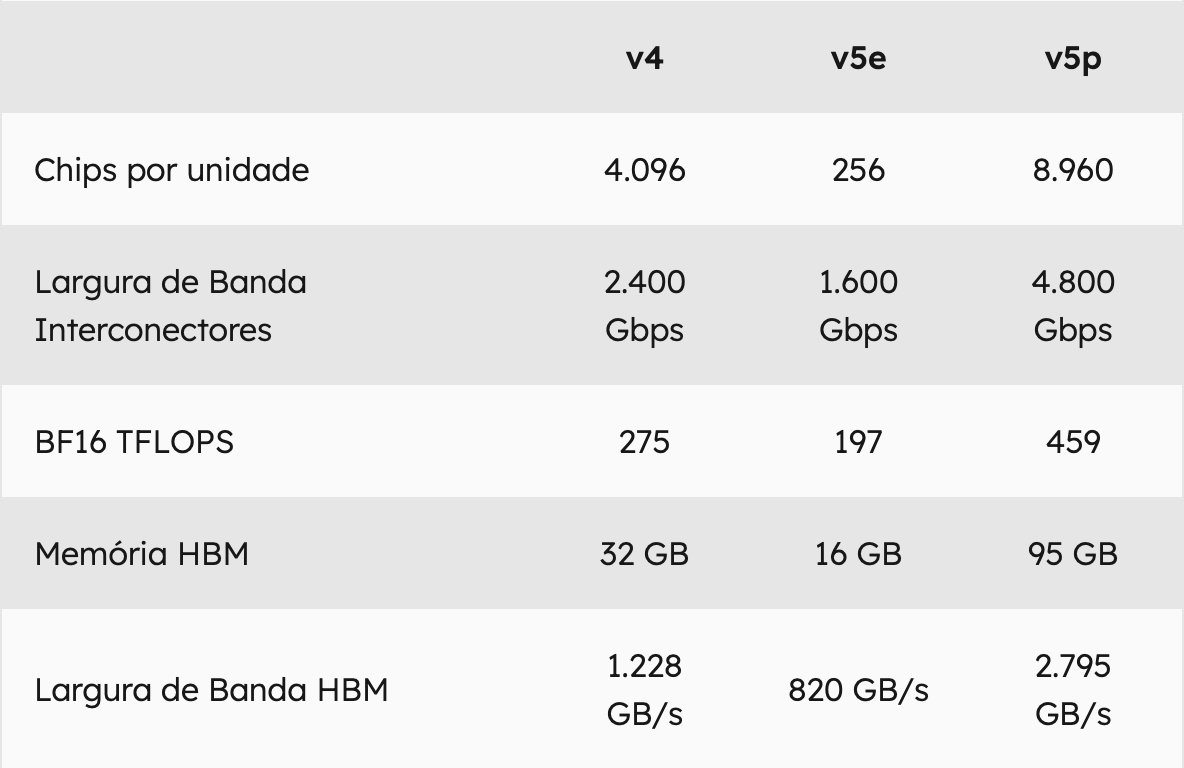
\includegraphics[scale=0.5]{comparativo-tpus}
\centering
\caption{Comparativo entre TPUs Google para cargas de trabalho em IA e LLM}
\end{figure}

Mas no fim, o que significam esses valores? A Google promete que a nova TPU consegue escalar o tempo de treinamento, sendo até $4X$ mais rápida que TPUs mais baratas, como a $V4$, devido ao dobramento no tamanho de operações em ponto flutuante que são entregues.

% --- CHAPTER 9 --- % 
\chapter{Google Colab e distribuição}

\bibliographystyle{alpha}
\bibliography{sample}

\href{https://www.run.ai/guides/cloud-deep-learning/google-tpu}{TPU e Arquitetura}

\href{https://cloud.google.com/blog/products/compute/performance-per-dollar-of-gpus-and-tpus-for-ai-inference}{Comparativos oficiais em modelos de IA (TPU vs GPU)}

\href{https://canaltech.com.br/inteligencia-artificial/cloud-tpu-v5p-e-o-novo-e-mais-poderoso-acelerador-de-ia-do-google-272299/}{TPU v5p}

\href{https://cloud.google.com/tpu?hl=pt-BR}{Conceitos básicos}

\href{https://en.wikipedia.org/wiki/Tensor_Processing_Unit}{Wikipedia, tem tudo}

\end{document}